\chapter{General Introduction}

\epigraph{\textit{Natural selection cannot possibly produce any modification in any one species exclusively for the good of another species.}}{--- \textup{Charles Robert Darwin}}

\minitoc[n] % minitoc without title

% We will volontarily be vague at time. Please bear with us

\section{The Evolution of Cooperation}

  \subsection{Cooperative Behaviours and their Importance in Evolutionary History}

    % Peut-être que je m'épanche un peu trop là quand même

    \subsubsection{The abundance of cooperation} When looking at the natural world, cooperation is one of the social interactions that seems to be the most prevalent in every level of nature's complexity. In particular, its examples and pratical occurences prove to be as diverse as central in numerous different species. As we will see in the next Subsections, many different definitions of what really constitutes a cooperative behaviour exist. In our case, we will choose the most basic one: cooperation is a behaviour where an \emph{actor} (the individual who initiates the behaviour) behaves in such a way that is beneficial to a \emph{recipient}~\parencite{West2007a}. In particular, this behaviour may or may not be costly for the actor and the actor might not even be aware of the recipient. Obviously, in most cooperative interactions more than two individuals are directly concerned. As such, it can sometimes even be as difficult to clearly define the actors and the recipients as extracting costs and benefits.

    As we previously stated, cooperation pervades every aspects of complexity in the living. For example, even unicellular organisms such as bacteria or microorganisms are known to frequently act in a cooperative manner. By using secreations, these organisms are capable of collective sharing and communication~\parencite{Elena2003, Keller2006, West2006}. For example, \emph{Pseudomonas aeruginoas} are known to engage in situations that are known as \emph{public goods games}~\parencite{Popat2012, Harrison2013}. In particular they are capable of producing nutrients that every organisms as well as themselves can enjoy in the vicinity. However, this also means that some organisms could profit from these nutrients without having to produce anything themselves (given that production is costly). This is wehre a problem of public goods can arise: because "cheaters"\footnote{The term "cheaters" will appear several times along the lines of this manuscript. Because this word has a particular bad connotation with regards to human actions, it may be misunderstood that we attribute a malevolent intention to the organisms. Rather, through the rest of the manuscript, It should be understood as "someone who profits from a benefit without paying any cost".} can benefit from these nutrients without contributing themselves. Interestingly, these situations are well studied in the realm of cooperative dilemma, as in economic research for example, which proves how complex these cooperative interactions in microorganisms are. It would also not be so far-stretched to consider that the complex network of genes interactions, where genes act together to build complex living machines may very well fall under the umbrella of cooperation. It is even more astonishing when we consider that those genes used to be independent replicators living freely~\parencite{Dawkins1976, Szathmary1995}. Finally, and in a similar fashion as our previous example, multicellularity is a perfect display of high cooperation between numerous different organisms. The birth of multicellular organisms is explained by the fact that single prokaryotic organisms gathered and where incorporated as mitochondries in what are now eukaryotic cells to form complex multicellular organisms. Szathmary \& Maynard Smith considered this cooperative transition to multicellularity as one of the major transitions in evolution~\parencite{Szathmary1995}.

    \begin{figure}[hbt]
        \begin{center}
          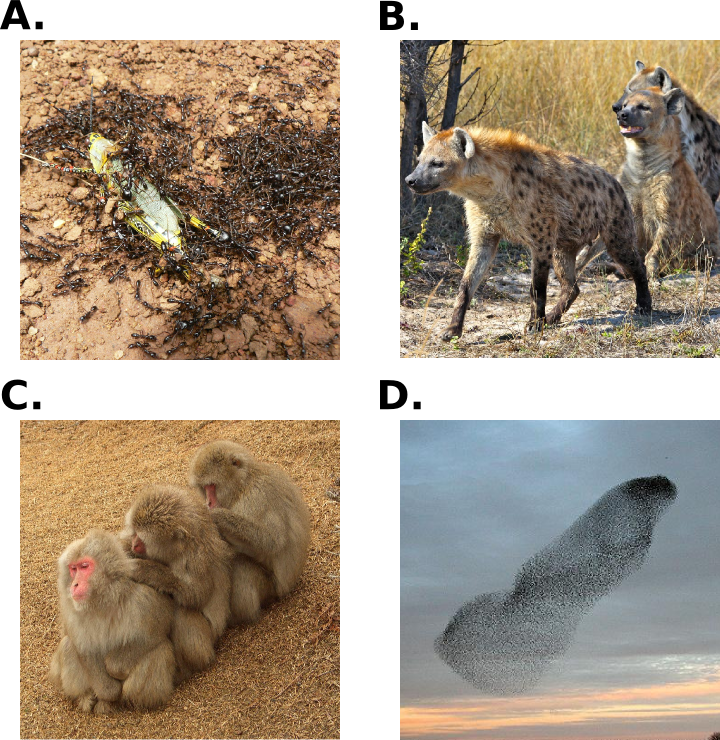
\includegraphics[scale = 0.5]{fig/Intro/CooperationExamples.png}
          \caption{\textbf{Cooperation at every level of complexity.} {\em (A)}~Eusocial insects like Hymenoptera (e.g. ants) are capable of impressive collective behaviours. {\em (B)}~Social carnivores exhibit strong cooperative behaviours and are capable of great feats of coordination during collective hunts. {\em (C)}~Social grooming is a social behaviour where individuals will groom each other reciprocally. It is thought to be a bonding exercise whose ultimate goal is to strengthen the social structure of the group. {\em (D)}~Flocks of birds are signs of the emergence of collective motions as if every individuals were part of a single bigger entity.} 
          \label{fig:CooperationExamples}
        \end{center}
    \end{figure}

    Much higher on the size scale is a popular textbook example of social behaviours: ants~(Figure~\ref{fig:CooperationExamples}~(A)). More generally, the presence of \emph{eusociality} in the animal world is an astonishing display of cooperative features~\parencite{Wilson1990}. While ants are among the most well-known examples, insects from the Hymenoptera (i.e. ants, wasps, bees) and Isoptera (i.e. termites) orders are all eusocial and represent most of the insect biomass\parencite{Wilson2008}. It is interesting to note that two rodent species, the naked mole-rat and the Damaraland mole-rat, are the only vertebrates to have achieved eusociality. Eusociality might be defined as one of the highest levels of sociality and displays several impressive examples of highly advanced cooperative actions. For example, there is cooperative care of youngs in eusocial societies, which means that individuals help raise offsprings which are not their own. Also, eusocial insects are capable of achieving efficient division of labour, a cooperative trait where individuals specialize between several roles, either to achieve several tasks simultaneously or to coordinate more efficiently. In particular, division of labour is often permanent and comes with strong morphological differences between specialized individuals. Last but not least, eusociality is also defined by the division of reproductive labor. This means that there exists reproductive and non-reproductive castes (e.g. the worker caste), which is an extreme form of cooperation between these individuals. Because of all of these reasons, an ants colony is often viewed as a particular superorganisms wherein individuals work as one for the benefit of the group.

    If we unzoom again the lens with which we look at the world, we can find other powerful examples of cooperation among bigger vertebrates. Numerous species have evolved strong sociality, or presociality, which gives the opportunity to watch impressive cooperative actions in the animal world. For example, social carnivores are capable of collective hunting, where several members of the same group will coordinate their actions to catch a particularly difficult or quick prey. For examples, lions are famously known for their communal and highly cooperative behaviours of collective hunting, for which they are capable of division of labour~\parencite{Scheel1991, Stander1992}. Less well-known but as much impressive, spotted hyenas~(Figure~\ref{fig:CooperationExamples}~(B)) also demonstrate high level of coordination in their collective hunting habits. While often wrongly considered but a scavenger, hyenas are also great hunters who rely on signaling and communication to coordinate~\parencite{Drea2009a, Smith2010, Smith2012a} and are capable of defending their catch against lions. The behaviours of those predators could easily be considered as complex tactics by a human observer. But even without being concerned with something as brutal as hunting, social carnivores tend to live, as their name suggests, in highly cooperative societies. To go on with the example of spotted hyenas, they are in particular considered to be the most social among Carnivora~\parencite{Mills2003} and the complexity of their social organization is comparable to that of primates~\parencite{Drea2003}. They live in a matriarchal societies where the females dominate the males and enforce the hierarchy through agression. Non-dominant females also take care of the youngs of other females higher in the hierarchy, something which is known as alloparenting and can also be found in primates~\parencite{Small1990} and in other carnivores~\parencite{Packer2001}. Among several social species, individuals also engage in social grooming~(Figure~\ref{fig:CooperationExamples}~(C)), where they will clean each other and which is an important bounding activity which strengthen the social structure of the group~\parencite{Spruijt1992}. Finally, we can also quickly mention the behaviours of sentinels, for example in birds like the Arabian babbler~\parencite{Wright2001} or meerkats~\parencite{CluttonBrock1999}. Individuals who adopt these behaviours will act as watchers for other individuals in their group, responsible for looking for predators approaching and warn the other individuals, sometimes thus taking the risk of attracting attention to themselves.

    It is also easy to be amazed by the collective motion of flocks of birds~(Figure~\ref{fig:CooperationExamples}~(D)). Animals might sometimes organize into flocks, herds or schools from which will emerge a collective behaviour~\parencite{Couzin2002, Couzin2003}. In particular, what is impressive is that the collective cohesion achieved is due to individual behaviours which do not depend on high cognitive abilities and does not require a particular central decision. These social behaviours are beneficial to the individuals that constitute the groups because it can for example increase group vigilance, confuse predators, decrease the risk for each individual to be attacked or even allow to organize an active defense against a predator~\parencite{Hamilton1971, Olson2013}.

    For the moment we simply gave examples of cooperation between members of the same species (intraspecific cooperation). Yet if we again look at a higher scale we can also observe numerous displays of cooperation between individuals of different species (interspecific cooperation). Often called mutualism (as we explain later), this form of cooperation is abundant~\parencite{Bshary2004}. For example, most plants require pollinators in order to transport their pollen so that they can succesfully pollinate the flowers. In exchange, the pollinators, whose most representative are insects, gain nectar as a benefit. Another example is that of cleaning symbiosis, where a "client" has its teeth or body cleaned from parasites or dead tissues by another smaller "cleaner"~\parencite{Poulin1996}. For example, some fishes, especially wrassers, are known to often clean other bigger fishes, to the point that there exists "cleaning station" where multiple aquatic animals converge to enjoy their services. The yellow-billed oxpecker also regularly eats insects and ticks from the back of mammals. The gut flora of some animals, human beings among them~\parencite{Backhed2005}, is also another example of strong interspecific cooperation, as it is constituted of up to 100 trillion of microorganisms that help process food.

    % KILLER WHALES ? Domestication ?

    % On peut en dire plus sur les humains mais j'ai pas les références pour le moment.

    In conclusion, in nearly every different levels of complexity in the living world, we can find examples of cooperative actions. More importantly, cooperation is not only present but also appears to be one of the leading factors in every major transitions in evolution~\parencite{Szathmary1995}. Moreoever, we did not touch upon human cooperation until now but it is obvious that human beings are very strong cooperators. In particular, cooperation is at the basis of the construction of our social structure and social sciences have been for long interested in studying human cooperation~\parencite{West2011a}. Therefore there is particular interest in trying to explain how could cooperation evolve and give rise to so much diversity in social behaviours today. 


    \subsubsection{Evolving cooperation} Yet explaining the evolution of cooperation has been one of the major challenges in evolutionary biology~\parencite{Hamilton1964, Dugatkin2002, West2011a}. Charles Darwin, as shown by the epigraph of this chapter, had already figured that the evolution of cooperation could pose a problem to his theory. In particular, he thought that the existence of a non-reproductive caste in eusocial insects, which we previously talked about, was "one special difficulty, which at first appeared to me to be insuperable, and actually fatal to my whole theory"~\parencite{Darwin1859}. 

    Indeed, the theory of evolution has it was stated by Darwin is often also called \emph{survival of the fittest}. Based on the theory, life is a struggle where only the fittest individuals survive. From this it stems that a particular trait can only be adaptive if it benefits its individual. The main purpose of evolutionary biology is to explain adaptation~\parencite{West2011a}. In particular, thanks to the work of Gregor Mendel on heritability, we know now with precision about how the process of emergence and spread of genes happens in nature. Namely, genetic material spreads through the reproduction of their host which means that the ultimate "goal" of a gene is to increase the reproductive capacity of the individual (something that Richard Dawkins called the "Selfish Gene"~\parencite{Dawkins1976}). Consequently, a trait can only be adaptive if it increases the relative number of offsprings (i.e. the fitness) of the individuals which expresses it. This is where the theory of natural selection seems to contradict the existence of cooperation. 

    In its simplest form, cooperation is defined as a behaviour that benefits another individual than the one expressing it. In some cases, a cooperative action can even decrease the relative fitness of an individual. For example, a individual that acts as a sentinel for the group takes the risk of being spotted more easily by a predator, thus paying a hefty cost for the good of the others. In particular, those individuals are under the threat of being invaded by cheaters (or freeloaders\footnote{The term "freeloader" has no malevolent connotation. It is simply used in the same way as the term "cheater" for which we discussed the meaning earlier.}). Indeed, let's imagine a population constituted of cooperators that can pay a certain cost to give a benefit to the other individuals (for example we can think about the example of \emph{P. aeruginosas} which we previously talked about). A given individual thus can benefit from every individuals in the population and this situation seems ideal. However, say now that a mutant, which does not cooperate, appears in the population. Then this mutant can benefit from the cooperative actions of others without having to pay any cost. From this it stems that its relative fitness will be higher than that of the other individuals. In consequence, it will produce more offsprings and mutants will begin to invade the population. The process will repeat itself as cheaters always have a higher fitness than cooperators until no cooperators are left in the population. From this comes that cooperation should not be able to exist. Biologists have therefore been studying the mechanisms which could explain the evolution of cooperation for several decades. Numerous models have been proposed to classify the different mechanisms which could explain the adaptation of cooperative traits (we direct an interest reader to a few of them~\parencite{Dugatkin2002, Keller2006, Bergmuller2007a, West2007}). For our overview of cooperation in this present manuscript, we follow the classification of West and colleagues~\parencite{West2007a}. In particular, these mechanisms can be classified in two main categories: \emph{direct fitness benefits} and \emph{indirect fitness benefits} (see Figure~\ref{fig:ClassificationCooperation}).

    \begin{figure}[hbt]
        \begin{center}
          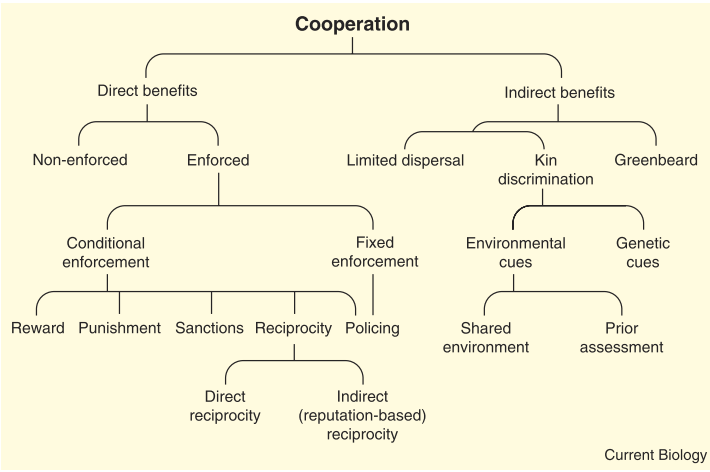
\includegraphics[scale = 0.50]{fig/Intro/ClassificationCooperation.png}
          \caption{\textbf{Classification of the mechanisms behind the evolution of cooperation.} Numerous classifications for the explanation of the evolution of cooperative actions have been proposed. However, most people agree that those explanatations can be divided into two categories: direct benefits and indirect benefits. Inside these two main categories, several mechanisms can be invoked in order to understand how cooperation could evolve and be maintained in a population. This picture was taken from the work of West and colleagues~\parencite{West2007}.} 
          \label{fig:ClassificationCooperation}
        \end{center}
    \end{figure}

  \subsection{Altruism and Indirect Fitness Benefits}

    A particular type of cooperative actions that has garnered great attention is the evolution of \emph{altruism}. We consider a behaviour to be altruistic when the actor of the behaviour pays a cost in an action benefitting another individual~\parencite{Hamilton1964, West2007a}. Please keep in mind that "costs" and "benefits" refer to the fitness of the individual (i.e. the number of this individual's offsprings) and not direct material elements. This is important because a cooperative action could be deemed altruistic in the short term and yet reveal to be beneficial to the actor in the long run. This was at the origin of several debates on the very definition of altruism which we will not talk about in this manuscript. We will simply here settled for the definition mostly admitted today of considering the costs and benefits on the lifetime direct fitness of the individuals, i.e. the impact on the production of offsprings~\parencite{West2007a, Lehmann2006}. From our general overview of cooperative actions in the previous Subsection, several (if not most) of our examples could be considered altruistic. For example, the costly secretion of nutrients by \emph{P. aeruginosas} corresponds, in its simplest form, to an altruistic action. The social behaviours of eusocial insects is also a major example of altruism in the natural world. In particular, the distribution of reproductive labour means that a part of the individuals do not reproduce at all, thus paying the highest fitness cost possible. Finally, the behaviour of sentinels, who take the risk of being spotted by a predator when they warn their conspecifics of this predator, may also appear altruistic.

    % Dire que bon c'est pas vraiment altruistic pour les sentinels ? Genre on peut considérer limite ça comme des mutual benefits

    The main problem posed by the evolution of altruism is its stability against the invasion of cheaters. As we previously said about the problem of cooperation, a population constituted of cooperators will be easily invaded by cheaters who profit from the benefits of cooperation without paying the costs. This leads to a population entirely constituted of cheaters, although the mean fitness of the population may be smaller than that of a population constituted of cooperators.

    This sparked numerous research on the evolution of altruism. The most well-known mechanism for the evolution of altruism was proposed by Hamilton: \emph{kin selection}~\parencite{Hamilton1964}. This mechanism conveys the idea that a particular trait can spread through the reproduction of relatives. If we consider the unit of selection in evolution to be the gene (as explained by Dawkins with his selfish gene~\parencite{Dawkins1976}), it does not really matter if a particular individual reproduces or not as long as the genetic material can spread one way or another. If an individual helps another individual that is genetically close to him (i.e. genetically related), he is still passing down its own genes even if he ultimately does not produce offspring. In consequences, an altruistic trait can still spread in the population through helping a relative who may possess this trait: this is kin selection. This general idea of the survival of one's genes through a relative is encapsulated into the concept of \emph{indirect fitness benefits}. Namely, if we consider that the goal of an individual is to spread its genes, then aiding its relatives contributes to its fitness. This wider definition of fitness is called the \emph{inclusive fitness}~\parencite{Grafen1984}, which is constituted of both the direct and indirect fitness benefits.

    The general concept of kin selection is nicely summarized by the popular \emph{Hamilton's rule}~\parencite{Hamilton1964} which states that an altruistic behaviour should be favoured if:

    \[br > c\]

    where $b$ and $c$ are respectively the benefits and costs of the cooperative behaviour and $r$ the genetic relatedness between the two individuals (i.e. how genetically similar are the two individuals compared to the rest of the population). To put it more simply, an altruistic trait can be selected if the benefits of this trait weighted by the relatedness to the individuals outweigh the cost of cooperating.

    While kin selection provides a nice framework for understanding the evolution of altruistic behaviours, it does not provide an explanation on how it is possible to generate sufficient genetic relatedness between individuals for kin selection to function~\parencite{West2007}. Several mechanisms have been proposed to allow kin selection to happen in nature (Figure~\ref{fig:ClassificationCooperation}). The first mechanism is the ability to recognize genetically related partners, also called \emph{kin discrimination}. In particular, kin discrimination can occur through either environmental (e.g. prior associations and living in shared environment) or genetic cues~\parencite{Grafen1990}. For example, long-tailed tits are known to discriminate between kins and non-kins by using vocal cues~\parencite{Russell2001, Sharp2005}. These vocal recognition signals are learned by the adults during the nesting period and the individuals will tend to help primarly individuals with whom they were associated during this nesting period. This causes long-tailed tits to help in the nest of relatives when they have not been able to produce offsprings. Then, and while evidence of its existence are rare, another mechanism is the green beard mechanism~\parencite{Hamilton1964, Lehmann2006}. Rather than focusing on the mean similarity between the individuals' genotypes, this mechanism relates to relatedness on a particular loci in the genotype. The main idea is that a particular gene could be deeply coupled with the "gene for cooperation" and help recognize cooperators at the same time (e.g. thanks to a particular phenotypical trait, hence the analogy to a green beard thanks to which cooperators could be identified~\parencite{Dawkins1976}). Then, cooperators would be more prompt to cooperate with those who express the same trait. However, this sort of mechanisms can easily be used by cheaters who then could profit from cooperators~\parencite{West2007}. A last popular mechanism for the occurence of kin selection is that of limited dispersal~\parencite{Hamilton1972, Griffin2003}. Under limited dispersal, relatives will tend to keep close to one another. What this means is that altruistic cooperation can be directed to any neighbours because those neighbours will tend be strongly related to the individual. Thus, even without any particular discrimination mechanism, it is possible to ensure kin selection.

    Finally, we need for the sake of completeness to quickly talk about the long time debate about the influence of \emph{group selection} on the evolution of altruism. In particular, the evolution of cooperation was not deemed worthy of studying for some time because it was thought that it could easily be explained by group selection~\parencite{Axelrod1981}. There have been two major branches of this theory, now called old and new group selection theory~\parencite{West2007a}. In the old group selection, it was considered that a cooperative trait could evolve because it was beneficial to a whole group. For example, let's consider that there are two groups in competition, one constituted of cooperators and the other of defectors, who reproduce and consume resources selfishly. Because defectors exploit their resources selfishly, they would go extinct when resources disappear. Thus the group of cooperators, and therefore cooperation, could survive because selection acted at the level of the group. This is why we may often hear the false idea that an individual will behave in a certain way "for the good of the species". While this particular theory of group selection was then dismissed as nonexistent~\parencite{MaynardSmith1976}, a new group selection theory arised. In this new theory, the main idea is that individuals interact in small groups, which exist inside a given population (whereas old group selection considered the whole population to be the group). Then, because interactions take place between a small number of individuals inside a group, then the emergence of cooperative traits can be favored. Since then, it has been shown that kin selection and new group selection are mathematically identical concepts~\parencite{Hamilton1975, VanBaalen1998, Gardner2007} and that it is generally easier to use the kin selection framework~\parencite{West2007a}.


  \subsection{Direct Fitness Benefits and Mutualism}

    But most of the cooperative actions do not fall under the umbrella of the indirect fitness benefits. In fact cooperation can also be directly beneficial to the actor~\parencite{Leimar2010}. In this case, both the actor and the recipient benefit from the cooperative behaviour and we then say that the behaviour is mutually beneficial~\parencite{West2007a}. Before we talk more thoroughly about this subject we must clarify some confusions that sometimes arise in the litterature~\parencite{Bergmuller2007a}. In particular, some have considered cooperation to only refer to mutually beneficial behaviours~\parencite{Trivers1985, Lehmann2006} in comparison to altruism. Here we consider the broader definition where cooperation includes both altruistic and mutualistic actions~\parencite{West2007a}. There is also some confusion about the definition of \emph{mutualism}. While it can be used to describe mutually beneficial actions or sometimes even cooperation as a whole (as previously explained), it may also refer only to interspecific mutualism. In the context of this thesis, we are mainly interested in intraspecific cooperation. As such, we will tend to follow the advice of West et al.~\parencite{West2007} and use only "mutually beneficial behaviours" rather mutualism throughout this manuscript.

    As with the indirect fitness benefits, several mechanisms could explain how cooperation can be adaptive through direct benefits (see Figure~\ref{fig:ClassificationCooperation}. For example these benefits can be enforced in a several different manners. An exhaustive review of enforcement is beyond the scope of this manuscript but we will quickly describe this mechanism to give a general overview of its influence. First, one way those benefits can be enforced is through reciprocal interactions~\parencite{Trivers1971}. Under reciprocity, individuals will tend to help those who have helped them in the past and thus provide mutual (albeit delayed) benefits. In this case, we talk about direct reciprocity. In comparison, with indirect reciprocity, an individual will tend to help an individual who is known to help others, hence the notion of "reputation-based reciprocity". It is interesting to note that, outside of humans, reciprocity is thought to be unimportant~\parencite{Dugatkin1997}. Other forms of enforcement (or coercion~\parencite{Clutton-Brock2002}) include rewards, punishment, sanctions and policing. These types of enforcement are common in humans~\parencite{Fehr2002} but also in a lot of different social animals. Hyenas for example enforce cooperation inside the group through suppressed reproduction. The dominant females in the group will attack lower ranking females if they get pregnant or even their cubs directly. They thus ensure that her offsprings (and those of a few other high ranking females) are the only youngs in the groupe. This way, they enforce cooperative care (alloparenting) of they youngs and thus increase their survival chances. Another nice example in order to understand the different ways in which cooperation can be enforced is that of the cleaner fishes we previously talked about. While they eat parasites from their client, their preference would be to eat the mucus and tissue of their client. In return, clients have several way to enforce cooperation (i.e. eat only the parasites): partner choice, which means that they go only to "good" cleaners, partner switching, which means they go to another cleaner and directly punishing the clean through agression~\parencite{Bshary2005}.

    % TODO: Dire que Trivers parlait d'altruistic reciprocity ou on s'en balance ?

    But what we want to study in the context of this thesis is the case where cooperation between individuals is not enforced. Rather, all individuals have a shared interest in cooperating. This is something which is often called \emph{by-product benefits}, conveying the idea that cooperation is a by-product from an otherwise self-interested action. For example, a large group of individuals entails higher chances of survival (against both the environment and predators) and an increase in the benefits from foraging or hunting. This leads individuals to have a mutual benefit in creating groups and societies, something which is known as group augmentation~\parencite{Bergmuller2007a} and has been well studied, for example in the case of meerkats~\parencite{Clutton-Brock2002}. A nice example of the selfishness of by-products was provided by Caraco \& Brown with the Mexican Jay~\parencite{Caraco1986, Dugatkin2002}. When there is food in large enough quantity, these birds will share foods with other individuals' offsprings. While this behaviour may appear altruistic at first, it can be explained by purely selfish motives. In particular, chicks beg loudly until they are fed, which might attract nearby predators. Thus, an individual may share food so that another individual's chicks do not attract the attention of predator to its own offsprings.

    Finally, as a conclusion, it is important to state that the differences between all these mechanisms are generally subtle and hard to differentiate. In particular, indirect and direct fitness benefits are not necessarily mutually exclusive and a behaviour can evolved thanks to kin selection but then its benefits can be generated through enforcement.

    % Prendre l'exemple des arabians babblers de Clutton-Brock2002 ?

  \subsection{Stability Versus Origin}

    It could be argued that the cooperative behaviours from which all individuals mutually benefit are trivial. In particular in the case altruistic behaviours, the stability of cooperation is under the constant threat of invasion by freeloaders. As such the main problem involved is to study their \emph{stability} against subversion by cheaters. In comparison, when benefits are mutual there does not seem to be any evolutionary puzzle in the same way as with altruism: once a mutualistic behaviour has evolved, there is no incentive to free-ride~\parencite{Forber2015}. While this may be true, this does not take into account the problem of explaining the origin of cooperation~\parencite{West2007}, where it may be difficult for a cooperative behaviour to spread initially. More precisely, focusing on the stability of the cooperative behaviour does not answer the question of how these cooperative behaviours could evolve in the first place, i.e. the \emph{bootstrap of cooperative behaviours}.

    In particular, there is a problem posed by the evolution of mutually beneficial behaviours when they require the evolution of coordination~\parencite{Alvard2001, Alvard2003, Drea2009, Leimar2003}. For example, the evolution of collective hunting is one that is based on interdependence between the individuals~\parencite{Tomasello2012}, which means that the collective success of the group is dependent on the coordination between every individuals. Because of this interdependence, the problem is not one of stability but of shared intention between participants. In consequence there is a fitness valley to cross where all the individual have to evolve coordination before they are able to reap the benefits of collective actions. To put it more simply, we face a \emph{chicken and egg dilemma}. For a cooperative trait to be selected, it needs to benefit the individual. In this case this benefit cannot be obtained unless every individuals coordinate. In consequence, all the individuals must have already evolved cooperation. There has thus been a recent shift in evolutionary biology toward the study of the origin of cooperation (in the case of mutualistic actions) rather than its stability (in the context of altruistic actions)~\parencite{Forber2015}.

    This problem was also defined by Calcott~\parencite{Calcott2007a} as the difference between the \emph{distribution of benefits} (i.e. stability) and the \emph{generation of benefits} (i.e. origin). When we are interested in the distribution of benefits, we focus on the final fitness benefits and costs. That is what we previously did when we tried to explain why altruistic cooperation is adaptive thanks to kin selection (i.e. indirect fitness benefits). But when we focus on the \emph{why}, we tend to abstract from the pratical interactions that take place in order to generate the benefits: we ignore the \emph{how}. The difference between the \emph{why} and the \emph{how} is something that is also known as \emph{ultimate} and \emph{proximate} explanations. This difference was mainly introduced by Niko Tinbergen~\parencite{Tinbergen1963, West2007a} who described the two complementary manners in which we could study animal behaviour:

    \begin{itemize}
      \item {We can study the mechanisms of behaviour to give the proximate explanations}
      \item {We can be interested in the fitness consequences of the behaviour and reveal the ultimate explanations}
    \end{itemize}

    Tinbergen illustrated this difference with the nice example of the black-headed gulls. In particular, these birds remove the eggshells from their nest. The proximate (or mechanistic) explanation is that individuals will more likely remove objects from the nest when they have frilly edges and are egg-coloured and feather-light. The ultimate explanation is that predator are this way less likely to spot their offspring. The conclusion is that both explanations are necessary so that we can fully understand this behaviour. Scott-Phillips and colleagues~\parencite{Scott-Phillips2011} had another way to summarize the difference between these two explanations: proximate mechanisms generate behaviours whereas ultimate functions explain why these behaviours are favored.

    In the case of the evolution of collective hunting, it is thus necessary to study the proximate as well as the ultimate explanations. In particular, because the evolution of coordination is necessary for the emergence of the collective behaviour (and thus cooperation), this means that the mechanistic constraints may have a crucial influence on the ultimate evolution of cooperation. To put it differently, we aim to show that the nature of the coordination behaviours is critical for the capacity to bootstrap cooperation. As previously said, the shift toward explaining the origin of cooperation is pretty recent. As such, few works have focused on the quality of the coordination behaviour (i.e. proximate explanations) which have mostly been considered as a black box~\parencite{Calcott2007a}. We want to show that, by doing as such, critical mechanisms are ignored.

    % TODO: Besoin de faire ressortir plus clairement la problématique ?



\section{Model and Method}

  Now that we have properly introduced the global question asked in this thesis, we are interested in presenting the methods with which our study has been conducted.
  
  \subsection{Game Theory and the Stag Hunt}

    It is classical to use abstract models to study the evolution of cooperation, as we will explain more thoroughly in Chapter~\ref{chapter:model}, where we will provide a more extensive review of models used to that end. Those models are advantageous because they consider general mechanisms and capture the relations between key factors. From purely computational models to spatial simulations, a considerable toolbox of models has been expanded during the past decades in order to increase our understanding of the evolution of cooperation.

    Among all these types of models, the most famous for studying cooperation dilemmas are game theoretical models. The basic idea is that each game represents a particular conflict between several (most often two) players. Each game is provided with a \emph{payoff matrix} whose goal is to indicate for each player, given her strategy and that of the other player, what is her expected reward. This way, the payoff matrix is used to describe the specificity of the game as a whole. Game theoretical models are well used in economy and some of them, like the \emph{Prisoner's Dilemma}, are even highly popular outside the scientific community. As such, evolutionary biologists have also been interest in using game theory as a way to study the evolution of cooperative behaviours. In the case of evolutionary biology, the general framework is called evolutionary game theory~\parencite{MaynardSmith1973}.

    In the context of this thesis, we are interested in a particular type of games: coordination games. In particular, the most well-known representent of coordination games is called the \emph{Stag Hunt}~\parencite{Skyrms2004}. Introduced by Jean-Jacques Rousseau and popularized by Brian Skyrms, this game follows a simple story (see Figure~\ref{fig:MatrixStagHunt})). Two hunters have the choice of either hunting a hare or a stag. Catching a hare is easy for any of the hunters and these prey are present in such availability that we can consider that hunting a hare has no influence on the other hunter's strategy. However, a stag represents a much harder prey to hunt so that both hunters need to cooperate if they want to reap the benefits of going for the stag. Finally, a stag is obviously much more rewarding than a hare. Thus there is a real incentive to cooperate but also a risk of trying to cooperate alone and thus being at a disadvantage compared to the other w.r.t. relative payoff. As for most game theoretical models, the exact payoffs are of no particular interest as long as the order between each situation is respected. In the case of stag hunt, the order for each hunter is as follows: successful cooperation on stag, hunting hare (whatever the partner's strategy) and failed attempt at cooperation.

    \begin{figure}[hbt]
        \begin{center}
          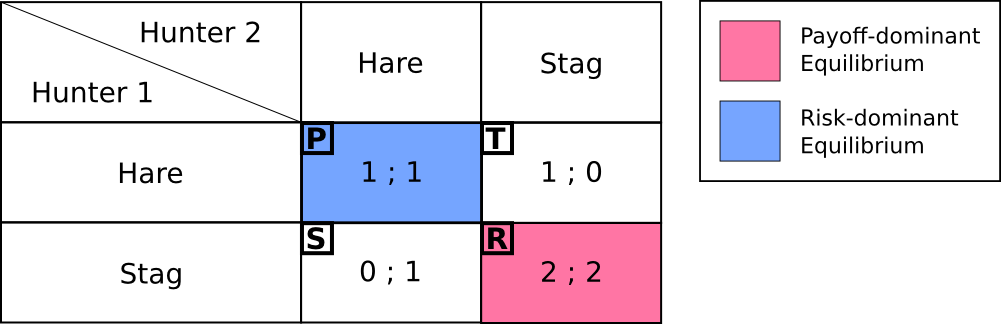
\includegraphics[scale = 0.50]{fig/Intro/StagHunt.png}
          \caption{\textbf{Payoff matrix of the stag hunt.} 
          In the stag hunt~\parencite{Skyrms2004}, we consider that during hunting, two hunters can either hunt a hare or a stag. Hunting a hare can be done in a solitary of cooperative fashion, which ensures that any individual who hunts gets a reward. In comparison, hunting stag can only be achieved in a cooperative fashion but rewards more than a hare. In consequence, an individual who would hunt a stag alone would not get any benefit from hunting. Payoffs are indicated in pair so that we have (Payoff for hunter 1; Payoff for hunter 2). The exact payoffs do not matter as long as the different situations are in that order: R (reward for cooperation) > T (temptation for defection) = P (punishment for defection) > S (sucker's payoff). The payoff-dominant equilibrium is the equilibrium where the hunters maximize their maximum payoff whereas the risk-dominant equilibrium is the one where they maximize their minimum payoff.} 
          \label{fig:MatrixStagHunt}
        \end{center}
    \end{figure}

    The particularity of this game is that there are two evolutionary stable Nash equilibria~\parencite{Nash1950, MaynardSmith1973}. This means that when both individuals hunt hare or when both individuals hunt stag, either strategy is stable against the invasion of mutants. More precisely, this implies that in comparison to the prisoner's dilemma, when the cooperative equilibrium is evolved (hunting stag), its stability is not threatened by the invasion of "defectors" (hare hunters). Thus, in coordination games, cooperation is stable when evolved but risky when rare~\parencite{Forber2015}. Consequently, this game can be used to model the problem of bootstrapping a cooperative strategy.

    But as previously said, when we abstract from the mechanics of behaviours as in game theory we choose to focus on the distribution of benefits at the detriment of the generation of benefits. To put it more simply, when we study the stag hunt we give no explanation on the origin of the coordination mechanisms which allow the individuals to reap the benefits of stag hunting~\parencite{Calcott2007a}. In particular, we tend to assume that the evolution of cooperation is coupled with that of coordination and that evolving cooperation is sufficient to be able to coordinate. In reality, cooperation cannot be beneficial unless coordination is evolved and coordination is not beneficial on its own.

    Our aim during this thesis is thus to model the pratical mechanics of coordination behaviours to study how they influence the ultimate evolution of cooperation. To this end, our approach is that of modeling in \emph{evolutionary robotics}\footnote{The choice of using evolutionary robotics is not without consequences and is not made randomly. In particular, there are critical reasons which justify that we use this technique rather than any other among the numerous modeling frameworks available for evolutionary biology. As this first chapter is a general introduction to this manuscript, we will motivate this choice in Chapter~\ref{chapter:model}}~\parencite{Nolfi2000}.


  \subsection{Evolutionary Robotics}

    Evolutionary robotics (ER) is a method based on designing robots by taking inspiration from natural evolution. In a particular, ER takes the concepts of \emph{selection} and \emph{variation} in order to simply the complex problem of designing a whole robotic systems. The idea of using evolutionary processes in order to solve engineering problems is now new. The whole field of evolutionary computing was created on this idea and still offers promising success in optimization problems where more classical methods fail~\parencite{Holland1975, Goldberg1989, Eiben2003}. Evolutionary robotics use the same principles to take on the complex task of designing part or all of a complete robot: sensors, morphology and control~\parencite{Nolfi2000, Floreano2008, Doncieux2015a}. Please keep in mind that the term "robot" is used loosely here and can refer either to a physical or simulated robot here. This does not impact the general method of evolutionary robotics.

    % TODO: Dire que l'EC c'est cool pour les black box trucs ?

    \begin{figure}[hbt]
        \begin{center}
          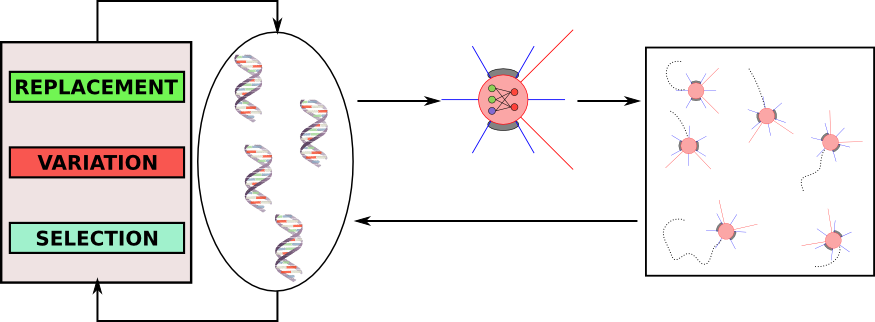
\includegraphics[scale = 0.50]{fig/Intro/EvolutionaryRobotics.png}
          \caption{\textbf{General workflow of an evolutionary robotics algorithm.}
          The main goal of ER is to evolve a population of genotypes. To that end, each genotype must be evaluated to obtain a fitness score. A genotype is thus translated into a phenotype (here an artifical neural network) and then embedded into a robot to act as its controler. The robot is situated in its environment and his behaviour is evaluated in accordance to the specifities of the task. Once every genotype has been asigned a fitness score, they undergo an evolutionary algorithm. This process select the genotypes deemed fit to create offsprings, on which variation is then applied. Finally this new population of genotypes replace the previous population and the process can go on for a new generation.} 
          \label{fig:EvolutionaryRobotics}
        \end{center}
    \end{figure}

    In particular, evolutionary robotics is constituted of an evolutionary algorithm whose goal is to evolve a population of artificial genotypes according to a fitness function (see Figure~\ref{fig:EvolutionaryRobotics}). While the actual format of the genotypes is of no particular interest here, it is but rarely similar to a real genotype in both complexity and features. Most often, each of these genotypes is a randomly generated collection of real values. This genotype is then translated into a phenotype which constitutes the robot's morphology and/or control. Again, the transition from genotype of phenotype as well as the actual phenotype itself can both vary greatly from one model to another. On that matter, one must choose what best fits his needs. The important point is that in ER this is the phenotype which is evaluated. To that end, the robot is situated into its environment and let to interact (with the environment and sometimes other robots). This principle of designing a robot in the context of its environment and the interactions it has with it is known as \emph{embodied intelligence}~\parencite{Pfeifer2007}.
    
    In the more classical models, a fitness function is used to compute the fitness score based on the behaviour of the robot in its environment. For example, in one of the first experiments where an evolutionary process was used to automatically design the control of a robot~\parencite{Floreano1994}, the goal was for a robot to navigate a looping maze. As such, the fitness function that had to be maximized was designed as follows:

    \[
      F = V(1-\sqrt{\delta v})(1-i)
    \]

    where (1) $V$ is the average rotation speed of the wheels, (2) $\delta v$ is the absolute difference between the speeds of the wheels and (3) $i$ the normalized maximum activation value between every sensors (where these sensors were infrared sensors capable of detecting obstacles). Thus, the goal of the robot was to (1) maximize its translational speed, (2) minimize its rotational speed and (3) minimze the activation of its sensors. So, to put it more simply, its goal was to move (1) as fast as possible (2) as straight as possible and (3) by avoiding obstacles at the same time. A large part of designing an evolutionary robotics algorithm is spent carefully crafting the fitness function to evolve the behaviour of the robot according to that desired (which is a challenge on its own).

    It is interesting to note that in those instances of evolutionary algorithm, fitness is thus used to guide the evolutionary process. This is obviously contrary to the biological definition of fitness which is an \emph{a posteriori} observation of the capacity to produce offsprings. While we will but briefly touch upon this subject in our manuscript, it is interesting to know that a few works in evolutionary robotics have been interested in this more "biologically realistic" approach to evolution. In the field of \emph{environment-driven} evolutionary robotics, multiple robots are evolved in open environments where the robotic agents need to encounter other agents so that they can exchange genetic material. Therefore, the selection pressures come from the environment and evolution is driven by the capacity to survive and produce offsprings rather than by a fitness score~\parencite{Ray1991, Bianco2004, Bredeche2010}.

    When every genotypes in the population have been evaluated, a selection scheme is applied based on the fitness score to decide which genotypes will be able to produce offsprings for the next generation. For example, a popular method to select the genotypes is to use \emph{tournament-based} selection. Under this scheme, an offspring results from a tournament between several (from one to the population size) randomly chosen genotypes in the population. These genotypes are then ranked by fitness score and each of the genotypes have a certain probability to be selected. Thus, given a certain probability $p$, the best ranked individual is chosen under probability $p$, then the second best ranked individual under probability $p(p-1)$ and so on. This process is repeated until the desired number of offsprings have been generated. Variation is then finally applied on these offsprings to create the population of the next generation. Variation can consist of mutations and/or crossover. A mutation is the process of randomly chosing one or several genes in the genotype, for example according to an uniform distribution, whose value is then randomly changed (in the way that depends from the format of the genotype). In comparison, the crossover is used to mix the genotypes of two different offsprings. In the most classical way to do crossover, one point crossover, a random point is selected in the genotype and genetic material is swapped between two individuals around this point. Finally, the population of the new generation is created and the evolution process can go on as long as needs be.

    Given the thematic studied in this manuscript, evolutionary robotics is interesting both as a modeling and design tool~\parencite{Trianni2014b, Doncieux2015a}. In particular, because what is evaluated are the phenotypes resulting from the evolved genotypes, this gives the possibility to really observe and study the behaviours evolved. Moreover, as the individual is embodied, we take into account all the interactions between this robot and the environment. This implies that we can study the coordination behaviours evolved in a qualitative fashion. Ecological features and particular mechanisms can then influence the evolution of these behaviours so that their implact on the evolution of cooperation can be thoroughly studied: the mechanics of behaviours are not considered as a black box anymore.



  \subsection{Experimental Setting}

    Now that we have presented both the game theoretical paradigm we take inspiration from and the artificial evolution method, we can finally describe our experimental setting. Please note that, as they may change depending on the exact experiments presented in this manuscript, some of the parameter values are not specified in this section.

    \subsubsection{Robot model} We want to study the evolution of simulated robotic agents (see Figure~\ref{fig:RobotModel}. These agents are capable of movement thanks to two independant wheels and are equiped with a collection of sensors. Those sensors are of two types: $12$ \emph{proximity sensors} and a $90$ degrees front \emph{camera}. On the one hand, the proximity sensors are equally distributed all around the robot's body and inform the agent about the proximity of any obstacle nearby (i.e. in a radius which equals twice of the body's diameter). On the other hand, the camera cannot recognize the obstacles but can feed the agent with the type of any objects it sees in the environment (including other agents). More precisely, this camera is composed of $12$ rays with an infinite range equally divided in the camera's angle. When one of these rays "sees" an object, the agent can know the type of this object and its proximity. The robot is thus constituted of simple sensory capabilities. The choice of having the robot model constituted of two different sensory feedback is not innocent. By dividing the sensory capabilities between the proximity sensors and the camera, we are essentially facilitating the process of evolving two basic capacities necessary for the robot: obstacles avoidance and agents recognition. This design is not to be considered as a realistic approach to evolution but rather as a way to ease the acquisition of basic skills that are of no particular interest here. Furthermore, while the obstacles avoidance mechanism is not expected to improve much during evolution, the appearance of cooperative behaviours in comparison should lead to variation on the manner with which to recognize agents.

    \begin{figure}[hbtp]
        \begin{center}
          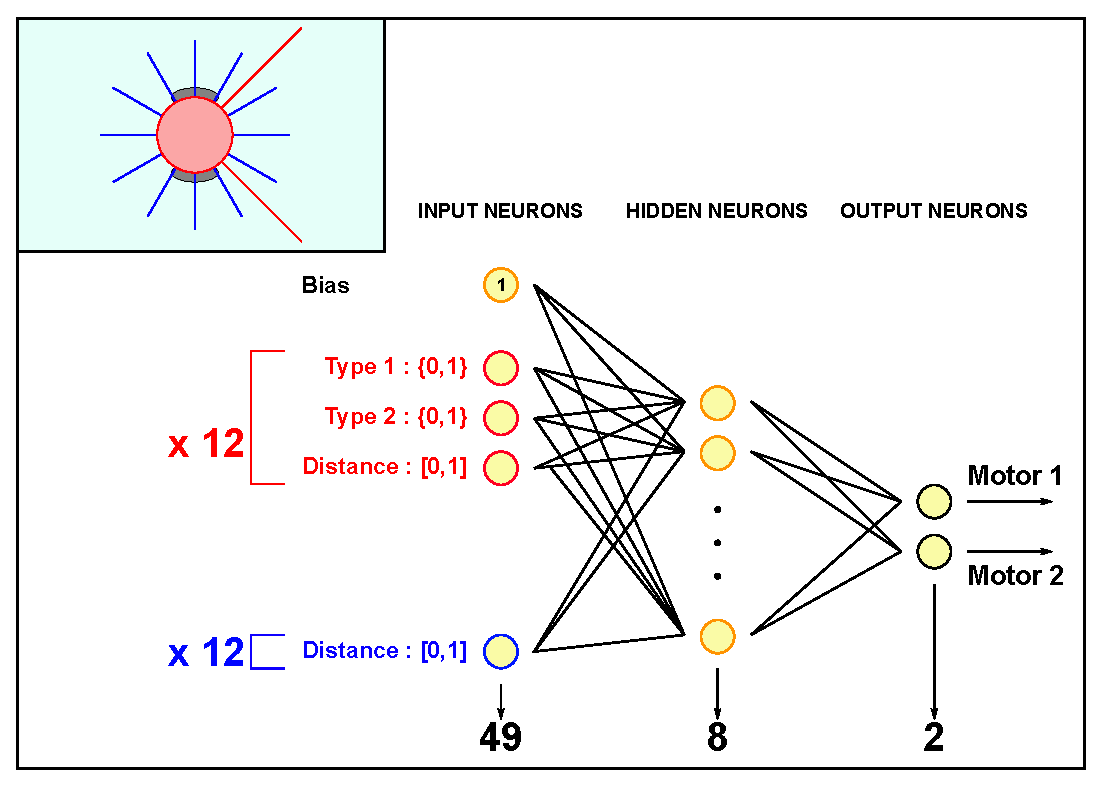
\includegraphics[scale = 0.60]{fig/Intro/RobotModel.eps}
          \caption{\textbf{Robot model of our experimental setting.}
          This figure represents the sensory and neural architecture of simulated robotic agent used in our experimental study. On the robot diagram, proximity sensors are represented by the blue lines whereas the front camera is shown as a red cone. The neural network is a multilayer perceptron with one hidden layer and whose inputs are constituted of all the sensory information of the individual. The outputs of the neural networks are the speeds of both of the robot's wheels.} 
          \label{fig:RobotModel}
        \end{center}
    \end{figure}

    \subsubsection{Controler} The controler of the agent is an artificial neuron network (ANN). While a lot of different types of controlers are used in evolutionary robotics, ANN are widely employed for their versatility~\parencite{Doncieux2015}. The principle behind a very basic neural network is that it is constituted of a layer of input neurons and a layer of output neurons which are connected (sometimes fully) to each other. Each one of the connection has a value, which is called a connection weight. The value of each output neuron is computed as the sum of the input neurons connected to it weighted by the connection weight. A transfer function can then be applied to this output to compute the final value. 

    In our case, we use a fully connected multilayer perceptron with one hidden layer. This neural network is composed of two outputs which are used to compute the speed of each of the robot's wheels. The inputs of the network are constituted of all the sensory information of the robot in addition to a bias neuron whose value is always $1$. This amounts to a total number of $49$ input neurons: $1$ for each proximity sensors, $4$ for each camera ray and $1$ for bias. The information of each camera is encoded by $4$ neurons as we use $2$ bits to encode the type of each object (hare, stag or the other agent) and $1$ last neuron for the proximity of this object. The hidden layer is constituted of $8$ neurons. Finally, the transfer function used in each neuron is a sigmoid and the topology of the ANN is never changed throughout evolution.

    \subsubsection{Environment} We place two evolved robots in an arena with four solid walls. This arena is filled with randomly positioned objects of different type, where the type can be recognized by the camera. These objects represent the prey that can be hunted by the individuals in the stag hunt game. The objects cannot move while the robots can move freely. In order to catch an object, an individual needs to move to this object and then stay next to it for a specified amount of time steps ($800$). After this duration, the object is removed from its position and replaced at another random position in the environment; we thus ensure a constant ratio of each type of object. For cooperation to occur, both robots need to be close to the object at the end of this duration. This thus implies that robots need to display actual coordination behaviours in order to be able to cooperate. This also means that an individual can reap the benefits of cooperation simply by being there at the very last step of the catching period.

    An object is always removed if an individual is next to it after this period of time, regardless of wether it requires cooperation. All that varies are the rewards given to the individuals. Please note that, even in the case of cooperation, we do not study the way rewards are distributed between individuals: they are both equally rewarded.

    \subsubsection{Evolutionary algorithm} The genotypes of the individuals is constituted of all of the connection weights of the neural network. Each gene is initially randomized in the interval where it takes its values, i.e. in \([0,1]\). To evolve these genotypes we use a very classical evolutionary algorithm. At each generation of the algorithm we evaluate each individual of the population in the arena presented before. Its partner is randomly selected in the population. To ensure that each individual encounters a fair sample of the population, each individual is separatly paired with $5$ different partners. Then a pair of individuals interact in the arena during a number of $20000$ time steps. In order to decrease the effect due to the stochasticity in the objects' random positioning, each pair plays $5$ different simulations. Thus, each individual plays a total number of $25$ simulations. Fitness is obtained by computing the average reward of the individual in these simulations.

    The individuals are then selected to produce offsprings. Throughout our experiments, we mainly studied two different selection methods: \emph{fitness proportionate} and \emph{elitist}. The former is the more classical one when modeling evolutionary biology because it corresponds to a Wright-Fisher model~\parencite{Wright1931} with constant population size. Under this model, we randomly sample through the population to select a parent to create each offspring that will constitute the population of the next generation. Each individual in the population has a higher probability to be selected if its fitness is higher. Each individual can also be selected several times. The latter selection scheme is also called a \((\mu + \lambda)\) evolution strategy. With this selection method, we always keep the $\mu$ best individuals of each generation for the next generation. Then we add $\lambda$ offsprings to the population of the next generation, where the parents of these offsprings are taken from the $\mu$ best individuals ranked by fitness score.

    % Justifier Elitist p/r à Fitprop ici ?

    Whatever the selection strategy, we always create the offspring in the same way. Each offspring is a mutated clone of its parent. Then mutation is applied independently on each gene according to the mutation rate. If a gene mutates, mutation is sampled according to a gaussian operator. We thus use no recombination (i.e. crossover) in any of our experiments.


\section{Evolving Coordination in Evolutionary Robotics}

  Until now, we have only introduced the general problem studied in this thesis. Namely, we claim that the proximate explanations of coordination behaviours have a criticial influence on the ultimate evolution of mutually beneficial cooperation. In particular, we believe that the nature of the coordination behaviour is of crucial importance if we want to fully understand the evolution of collective actions. This is what we consider to be the main thematic of the manuscript. 

  However, while this introduction was focused on the biological aspect of cooperation and the problem its origin and stability pose for evolutionary biology, we want to study several facets under this general thematic. In particular, our approach in evolutionary robotics entails that the contributions of this thesis can serve different purposes. Historically, evolutionary robotics has been used at its inception for the automatic design of robotic systems. However, there has been a real problem on how could the works in this field really contribute to scientific research as well as to whom it may be of interest~\parencite{Trianni2014b, Doncieux2015a}. It is now admitted that reseach in evolutionary robotics should be clearly directed toward either of two goals: modeling biological questions or designing robots~\parencite{Trianni2014b}. In this thesis, our goal is to present different contributions which separately aim for each of these goals. We want to quickly introduce each of these goals here to serve also as an introduction to each of the two parts of this manuscript.

  
  \subsection{Modeling the Evolution of Coordination}

    In the first part of this manuscript, we are interested in using evolutionary robotics so that we can model the evolution of cooperation. In particular, as we previously touched upon we want to show that, because we tend to generally ignore or minimize the pratical mechanics of behaviour, the role of coordination in the evolution of collective mutualistic actions is often underestimated. We thus study how the nature of coordination behaviours and the mechanisms that underlie their evolution may influence the ultimate evolution of cooperation. The particular issue we address here could be summarized as follows: \emph{what are the mechanisms which influence the proximate causes of coordination behaviours and facilitate the ultimate bootstrap of mutualistic cooperation ?}

    %TODO: un moyen de faire mieux ressortir la problématique ?

    To that end, we will spend some time in the introduction of this part to really motivate our choice of using evolutionary robotics, something we deliberately skipped in this general introduction. In particular, one reason why the proximate causes of coordination have often been overlooked is that the classical models used for studying evolutionary problems may not be appropriate for this particular goal. We believe that among the distinct assumptions made by these model, some are critical if we plan to fully understand the evolution of coordination. However, it is important to make clear that we do not pretend our approach to be a more realistic depiction of nature. Rather we claim that, while we still study a theoretical abstraction of cooperative actions, the assumptions behind our model allow us to study particular mechanisms we believe of importance for this issue.


  \subsection{Designing Cooperative Robots}

    In the second part of the manuscript, we want to study the evolution of cooperation in a team of heterogeneous robots. In consequence, we focus on the automatic design of a multirobots system. As we will explain more in details in this dedicated part, multirobots systems have now been investigated for a long time for their advantages other single robots. In particular, they may allow to design more efficient and cheaper robotic systems as well as benefit from the redundancy of multiple robots to design more robust systems. Moreoever, it can simply sometimes be necessary to coordinate several robots at the same time to achieve a particular task. The pratical applications of such systems are numerous, in particular in environments where humans cannot go and where using a single and generally more complex robot would simply not be reliable enough. For example, cooperative robots could be used to investigate and perform reparation repairs inside nuclear plants after particularly catastrophic incidents. One could even imagine that it would be useful to send a group of robots to Mars, where robustness is critical and on site repairs are simply not an option.

    However, designing this sort of systems is hard. It is one thing to engineer a factory robot which is programmed to perform a very specific and repetitive task in a controled environment. It is another to design a robot capable of acting in an uncertain environment and able to adapt to the unexpected. And even more complicated when multiple robots must both possess these qualities expected from a single robot and also coordinate in an efficient way. As we will talk about in this part multiple automatic designing techniques have been proposed, in particular for the control of robots. However, when it comes to adaptability to changing environment and uncertainty, the "easiest" way is to design a robot that is capable to learn from previous experiences. In our case, even if considering an evolutionary process to be a particular learning technique is open to debate, we chose evolutionary robotics as a way to design cooperative robots. As for choosing evolutionary robotics to model biological problems, this choice will be dutifully justified in this part of the manuscript. 

    We can however quickly point out that our goal here is to also take inspiration from the results of our modeling of the evolution of coordination. In particular, we are interested in the nature of the coordination behaviours that could be evolved between heterogeneous individuals. Heterogeneous teams of robots allow for more diverse behaviours to emerge inside a group of individuals. However, while there has always been a clear interest on adding heterogeneity in multirobots systems~\parencite{Parker1994, Parker2008}, most research on the evolution of cooperative robots have been focused on homogeneous groups of individuals~\parencite{Waibel2009}. This is indeed one of the safiest way to ensure that robots will indeed evolve a cooperative behaviour, as there is no selfish interest to act in a solitary fashion. However, we believe that the influence of heterogeneity on the quality of the coordination behaviours is as much of importance as the capacity to evolve a cooperation solution. Thus, the issue we focus on in this second part of the manuscript is: \emph{how can we evolve efficient coordination behaviours in a group of heterogeneous cooperative robots ?}
